%%%%%%%%%%%%%%%%%%%%%%%%%%%%%%%%%%%%%%%%%
% Wenneker Assignment
% LaTeX Template
% Version 2.0 (12/1/2019)
%
% This template originates from:
% http://www.LaTeXTemplates.com
%
% Authors:
% Vel (vel@LaTeXTemplates.com)
% Frits Wenneker
%
% License:
% CC BY-NC-SA 3.0 (http://creativecommons.org/licenses/by-nc-sa/3.0/)
% 
%%%%%%%%%%%%%%%%%%%%%%%%%%%%%%%%%%%%%%%%%

%----------------------------------------------------------------------------------------
%	PACKAGES AND OTHER DOCUMENT CONFIGURATIONS
%----------------------------------------------------------------------------------------

\documentclass[12pt]{scrartcl} % Font size

%%%%%%%%%%%%%%%%%%%%%%%%%%%%%%%%%%%%%%%%%
% Wenneker Assignment
% Structure Specification File
% Version 2.0 (12/1/2019)
%
% This template originates from:
% http://www.LaTeXTemplates.com
%
% Authors:
% Vel (vel@LaTeXTemplates.com)
% Frits Wenneker
%
% License:
% CC BY-NC-SA 3.0 (http://creativecommons.org/licenses/by-nc-sa/3.0/)
% 
%%%%%%%%%%%%%%%%%%%%%%%%%%%%%%%%%%%%%%%%%

%----------------------------------------------------------------------------------------
%	PACKAGES AND OTHER DOCUMENT CONFIGURATIONS
%----------------------------------------------------------------------------------------

\usepackage{amsmath, amsfonts, amsthm} % Math packages

\usepackage{listings} % Code listings, with syntax highlighting

\usepackage[english]{babel} % English language hyphenation

\usepackage{graphicx} % Required for inserting images
\graphicspath{{Figures/}{./}} % Specifies where to look for included images (trailing slash required)

\usepackage{booktabs} % Required for better horizontal rules in tables

\numberwithin{equation}{section} % Number equations within sections (i.e. 1.1, 1.2, 2.1, 2.2 instead of 1, 2, 3, 4)
\numberwithin{figure}{section} % Number figures within sections (i.e. 1.1, 1.2, 2.1, 2.2 instead of 1, 2, 3, 4)
\numberwithin{table}{section} % Number tables within sections (i.e. 1.1, 1.2, 2.1, 2.2 instead of 1, 2, 3, 4)

\setlength\parindent{0pt} % Removes all indentation from paragraphs

\usepackage{enumitem} % Required for list customisation
\setlist{noitemsep} % No spacing between list items

%----------------------------------------------------------------------------------------
%	DOCUMENT MARGINS
%----------------------------------------------------------------------------------------

\usepackage{geometry} % Required for adjusting page dimensions and margins

\geometry{
	paper=a4paper, % Paper size, change to letterpaper for US letter size
	top=2cm, % Top margin
	bottom=2cm, % Bottom margin
	left=2cm, % Left margin
	right=2cm, % Right margin
	headheight=0.75cm, % Header height
	footskip=1.5cm, % Space from the bottom margin to the baseline of the footer
	headsep=0.75cm, % Space from the top margin to the baseline of the header
	%showframe, % Uncomment to show how the type block is set on the page
}

%----------------------------------------------------------------------------------------
%	FONTS
%----------------------------------------------------------------------------------------

\usepackage[utf8]{inputenc} % Required for inputting international characters
\usepackage[T1]{fontenc} % Use 8-bit encoding

\usepackage{fourier} % Use the Adobe Utopia font for the document

%----------------------------------------------------------------------------------------
%	SECTION TITLES
%----------------------------------------------------------------------------------------

\usepackage{sectsty} % Allows customising section commands

\sectionfont{\vspace{6pt}\centering\normalfont\scshape} % \section{} styling
\subsectionfont{\normalfont\bfseries} % \subsection{} styling
\subsubsectionfont{\normalfont\itshape} % \subsubsection{} styling
\paragraphfont{\normalfont\scshape} % \paragraph{} styling

%----------------------------------------------------------------------------------------
%	HEADERS AND FOOTERS
%----------------------------------------------------------------------------------------

\usepackage{scrlayer-scrpage} % Required for customising headers and footers

\ohead*{} % Right header
\ihead*{} % Left header
\chead*{} % Centre header

\ofoot*{} % Right footer
\ifoot*{} % Left footer
\cfoot*{\pagemark} % Centre footer
 % Include the file specifying the document structure and custom commands

%----------------------------------------------------------------------------------------
%	TITLE SECTION
%----------------------------------------------------------------------------------------
\usepackage{float}
\title{	
	Final project report
}
\usepackage{hyperref}
\usepackage{float}
\usepackage{xcolor}
\lstset{
    columns=fixed,       
    numbers=left,                                        % 在左侧显示行号
    frame=none,                                          % 不显示背景边框
    backgroundcolor=\color[RGB]{245,245,244},            % 设定背景颜色
    keywordstyle=\color[RGB]{40,40,255},                 % 设定关键字颜色
    numberstyle=\footnotesize\color{darkgray},           % 设定行号格式
    commentstyle=\it\color[RGB]{0,96,96},                % 设置代码注释的格式
    stringstyle=\rmfamily\slshape\color[RGB]{128,0,0},   % 设置字符串格式
    showstringspaces=false,                              % 不显示字符串中的空格
    language=c++,                                        % 设置语言
}
\author{Yuan Jiahao 2019010070} % Your name

\date{\normalsize\today} % Today's date (\today) or a custom date

\begin{document}

\maketitle % Print the title

%----------------------------------------------------------------------------------------
%	FIGURE EXAMPLE
%----------------------------------------------------------------------------------------

\section{Introduction}
\subsection{What is Sparse Deep Neural Network GraphChallenge?}
GraphChallenge encourages community approaches to developing new solutions for analyzing graphs and sparse data derived from social media, sensor feeds, and scientific data to enable relationships between events to be discovered as they unfold in the field.
\subsection{What problem to solve?}
A large tall matrix A,whose density is about 10.4\%, matrix multiplies with B,whose density is about 3.1\%,and different in every cycle,then copy the result to A.The cycle calculation will be done 120 times.

The problems seems like using a huge model contributed by 120 fully connected layers to predict 60000 samples.And require us to optimize the running time.
\subsection{Optimization Route}
The problem could be separated into 2 main problems:Which computation kernel to choose and How the task to be separated and distributed.

So we will focus on these two topics in this report.
\section{Computation Kernel}
Since a lot of research on MPI,openMP,CUDA,etc have been made in previous homework,writing a kernel by myself from scratch and exceed the library seems to be a not smart choice.So much more focus will be made on choosing function provided by CUDA kits.

For GPU,three ways have been chosen to be tested,just as the graphs followed.
\begin{figure}[H]
    \centering
    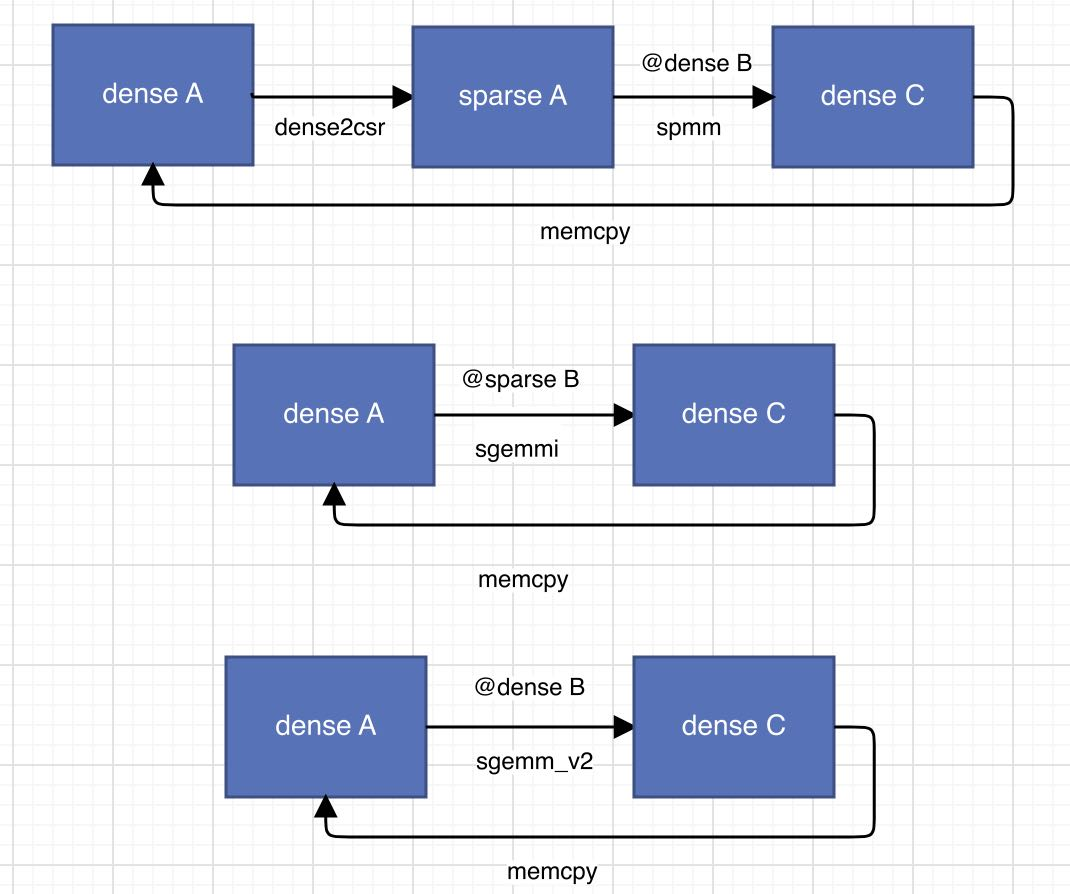
\includegraphics[width=0.6\textwidth]{p4.jpg}
    \label{}
    \caption{three tested GPU kernel}
\end{figure}
The first and second ways rely on library cuSparse,since I didn't found a sparse@sparse=>sparse function in the official documentation website.

In fact,the first one even rely on another function counting the number of zeros in the dense matrix,and then the dense2csr function could be called.Thus the transformation cost was tremendous,completely overridden time saved by sparse matrix multiplication.

So,what about the second one?It seems that the second one don't have any transformation cost. However,the whole computation still cost about 9500ms.And the last one,which calls cuBLAS library only cost about 6500ms.So maybe we have no choice but cuBLAS.I guess this is due to the density of B is too high,although 3\% sounds like a small number,but you have to realize that control is not free.

When it comes to CPU,since CPU has much more control ability,maybe it has better performance at sparse than GPU.However,for my poor parallel programming skill,the program works not very well.So I have no choice but openBLAS.
\section{Task Distribution}
\subsection{Splitting problem}
So,how can we split the problem and distribute it between CPU and GPU?

My initial idea was split matrix B by columns into B1 and B2,and then calculate A@B1 by CPU,A@B2 by GPU,finally merge them and goto the next cycle,like the graph below.
\begin{figure}[H]
    \centering
    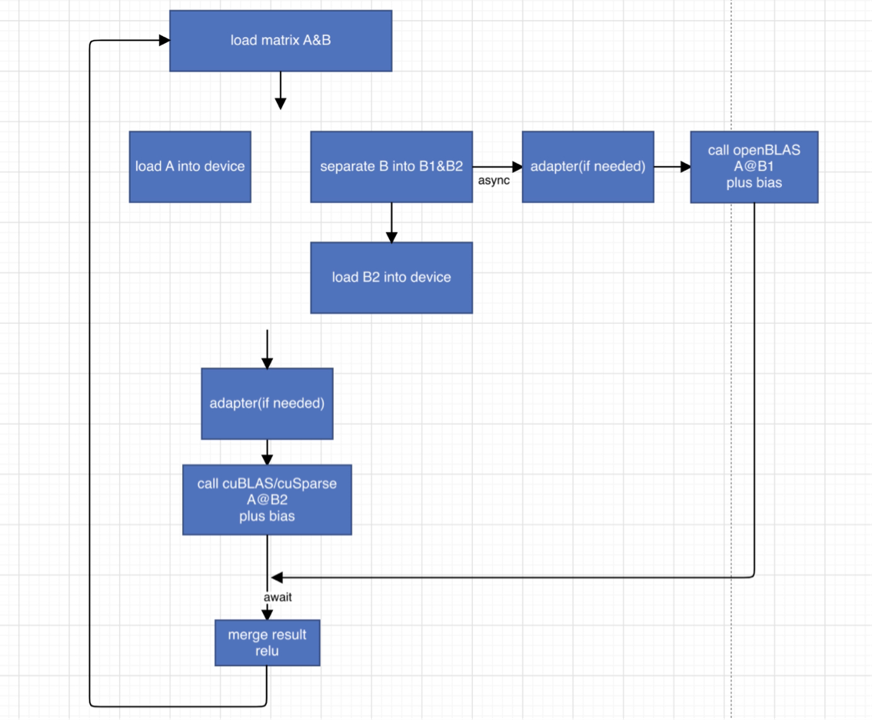
\includegraphics[width=0.8\textwidth]{s1.png}
    \label{}
    \caption{initial idea}
\end{figure}

And this design has a great problem,that every cycle either CPU or GPU will need to wait another one,and we need to copy data between CPU memory and GPU memory.IO is expensive,I dislike it.

So,why don't we split matrix A?Just split matrix A by rows into A1 and A2,and the Computation cycle can be done separately.The only thing we have to do is merge the final result,there is no need to do any memory copy between CPU and GPU during the calculation.

This idea also makes the problem into a completely liner problem,just like bitcoin mining.You know,bitcoin mining is seeking for a specific nonce(number once) from a large range.So it's a complete liner problem could be split and execute in a cluster or lots of single machines.So is our matrix multiplication.
\subsection{Distribute task between CPU and GPU}
Anyway,we have to test our CPU and GPU distribution design first.The matrix A was separated into two pieces,one for CPU and one for GPU.And the boundary was adjusted for the best diversion.However,the result was not good.CPU hardly come up with GPU when the boundary is 1000,which means GPU 59000 rows and CPU 1000 rows.And the worst thing is that the CPU calculation slowed down GPU.I will show you the contrast below:
\begin{figure}[H]
    \centering
    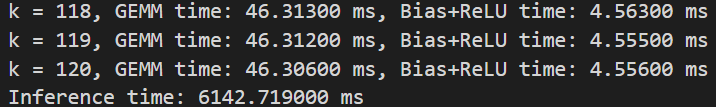
\includegraphics[width=0.8\textwidth]{j1.png}
    \caption{only GPU}
    \label{}
\end{figure}
\begin{figure}[H]
    \centering
    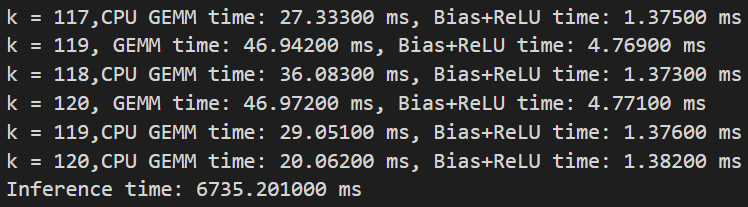
\includegraphics[width=0.8\textwidth]{j2.png}
    \caption{GPU 59000 and CPU 1000}
    \label{}
\end{figure}

The reason might be that GPU still need CPU to control something,maybe?And the full use of CPU makes the GPU be slowed down.But the most suspicious one is the cudaDeviceSynchronize function call in GPU calculation cycle.I tried to remove this one and make the whole calculation cycle into \_\_global\_\_ function so that the GPU will do this task completely independently.Although,some user at stackoverflow said at the latest version the cuBLAS already supports function call from GPU,but might due to the version of CUDA kit or something,function call at \_\_global\_\_ function told me it's not legal.
\subsection{Distribute task between nodes}
Anyway,it seems that it's no longer possible to distribute the problem between CPU and GPU.SO,what about distribute between nodes?I remember that teacher Liu mentioned cluster with 2 nodes and 4 GPU.Maybe it's possible to distribute the work between nodes.
\subsubsection{Communication}
To realize this idea,we need to solve the first problem,communication between nodes.Google told me that MPI can do things like that,but requires a lot work done by root,which I don't think is a good choice.So FFI(Foreign Function Interface) was my initial choice,which means using a glue process (here is Deno script written in TypeScript),communicating with other nodes and then calling the function in dynamic library.The architecture seems like this:
\begin{figure}[H]
    \centering
    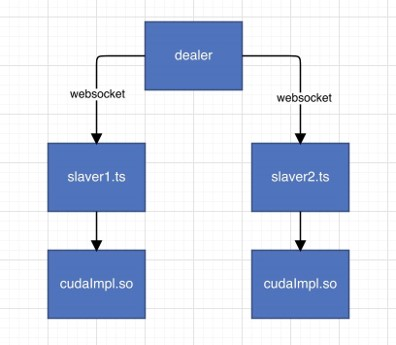
\includegraphics[width=0.5\textwidth]{ss1.jpg}
    \caption{initial architecture}
    \label{}
\end{figure}

Since C language doesn't have any runtime,requires us allocate memory and GC(garbage collection) by ourselves,which will be a trouble.Also,when we face random length message,complex message like JSON,C language will be a great trap for our programming.So,I initially was considering FFI at first.Since function will be very little,the majority cost being the calculation,I don't think it will cause too much performance loss.

And what about WebSocket?I don't want to discuss it too much in this report since it matters very little.Just give you an insight into its frame definition.
\begin{figure}[H]
    \centering
    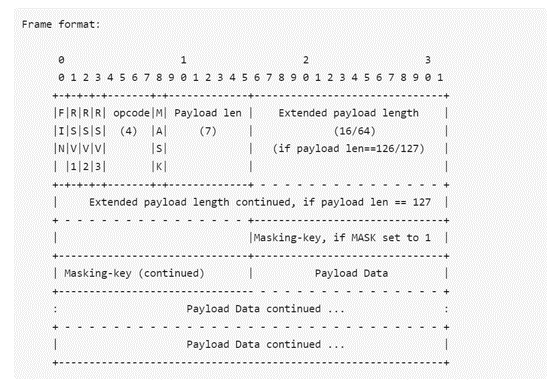
\includegraphics[width=0.75\textwidth]{ss2.png}
    \caption{frame definition}
    \label{}
\end{figure}

From this frame definition,you will find status,handshake,package length,etc,everything will be handled well by WebSocket.Also,it's a persistent connection protocol implement,so there will be no handshake cost transmitting data.

However,the problem is that nvcc compiler already added some glue into the compile output,which makes the shared library not executable.

After a very long struggle,it seems that it's not possible to realize this architecture.The only choice is make communication by C language itself.I actually tried some library,but all failed,so finally we have to do it ourselves.

So first,what's the message frame definition?Considering data needed to convey,which is taskId, clientId,message type,and the final result,maybe just a int32 array is ok.The first four byte is message type,and if the message is a result frame,the 5-8 byte is taskId,and the rest is result to merge.Also, there will be a message end symbol at the end.So,you can see my message constant definition as below:
\begin{figure}[H]
    \centering
    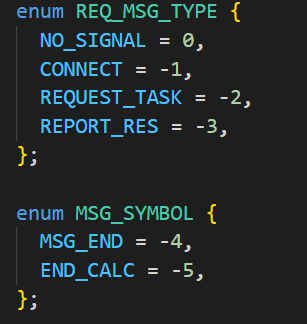
\includegraphics[width=0.4\textwidth]{def.png}
    \caption{message constant definition}
    \label{}
\end{figure}
That's another reason I gave up uint32,since negative number could be used as specific symbol.All the message will be transferred by socket.

Meanwhile,to ensure the socket communication not blocking calculation,two threads was created,that one for communication and another for calculation.They communicate by some pointer pointed to the same memory space,the variables are called requestTask and taskId.When the calculation thread comes to cycle 115th,requestTask will be set 1,and the communication thread will request the next taskId previously.

You will get a much more deep insight from my original code,but I will show you a short previous right now:
\begin{figure}[H]
    \centering
    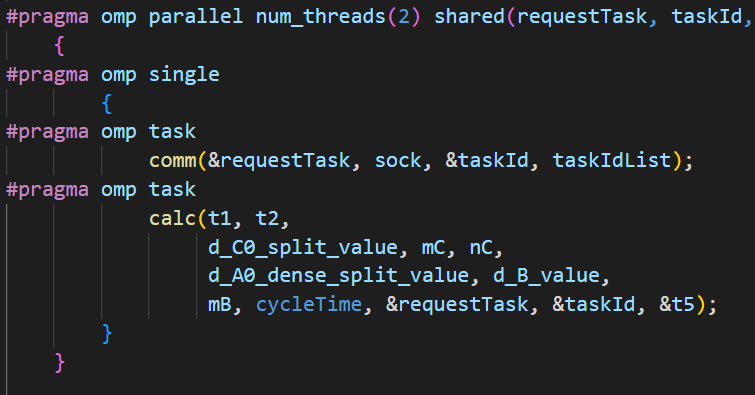
\includegraphics[width=0.8\textwidth]{ssss.png}
    \caption{two threads}
    \label{}
\end{figure}
\begin{figure}[H]
    \centering
    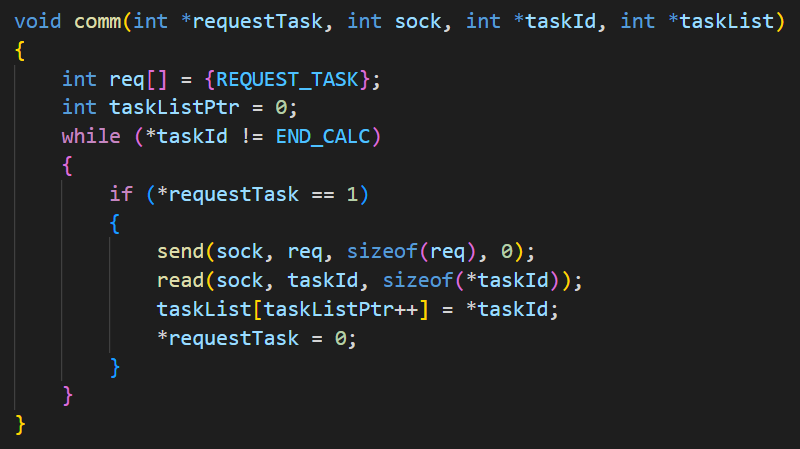
\includegraphics[width=0.8\textwidth]{sock.png}
    \caption{how the communication is made between nodes and threads}
    \label{}
\end{figure}
\subsection{Distribute tasks}
Finally,we come up to task distribution.In this section the only thing we have to do is expose a socket that controls the salver processes.So,how to implement it is our freedom.I choose Deno script written in TypeScript(which didn't realized before).All the message will be resolved by the event loop at the end of file deno.ts:
\begin{figure}[H]
    \centering
    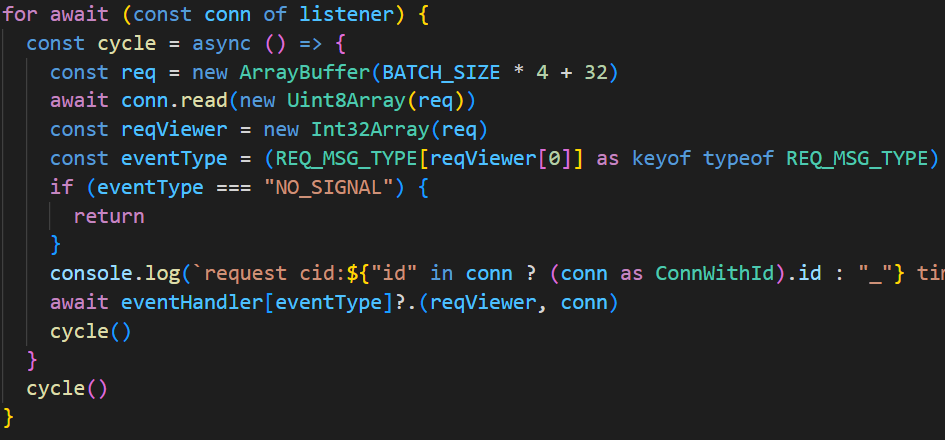
\includegraphics[width=0.8\textwidth]{loo.png}
    \caption{event loop}
    \label{}
\end{figure}

A const definition was made at the head of file(both main.cu and deno.ts),which controls the max device and batch size(batch size is dividing matrix A by how many rows).In fact the max device makes no sense since any node can come in at anytime,just give it a task.But our project requires the time consumption data.This const helps the dealer process knows how many nodes registered and start to distribute the task.Just like the code below:
\begin{figure}[H]
    \centering
    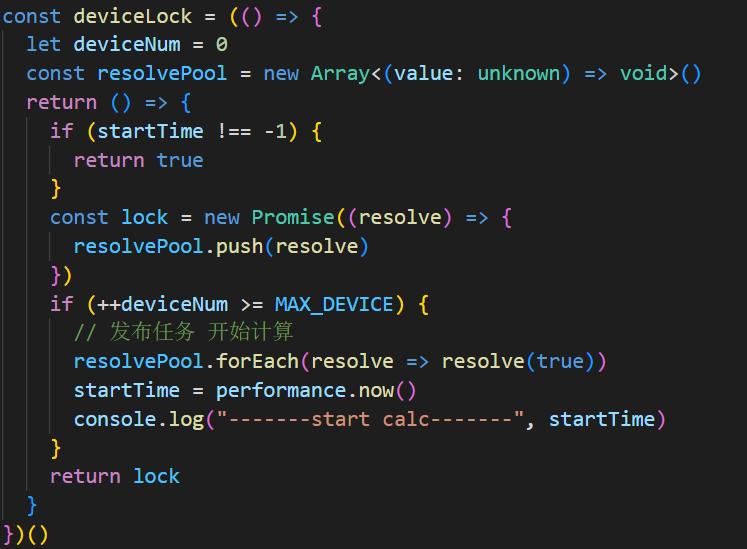
\includegraphics[width=0.8\textwidth]{lock.png}
    \caption{device lock}
    \label{dd}
\end{figure}
\begin{figure}[H]
    \centering
    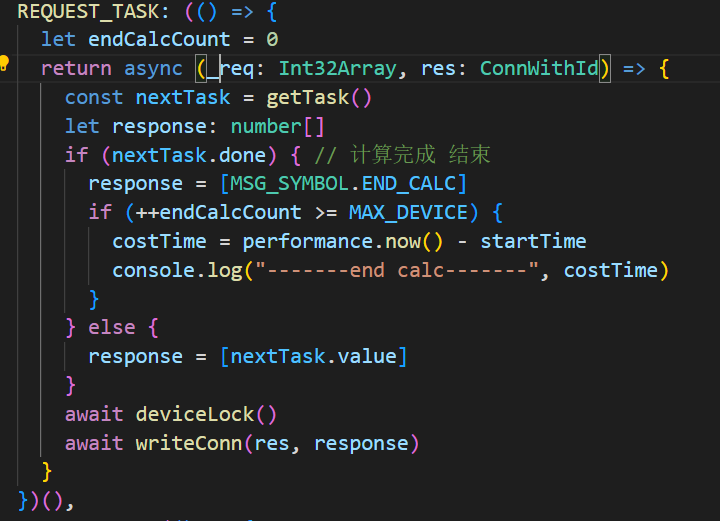
\includegraphics[width=0.8\textwidth]{han.png}
    \caption{response handler}
    \label{rr}
\end{figure}
From figure \ref{rr} will we find each request for task will be hang on until the async deviceLock function return a value.And only if all devices have requested the task,will this lock return value(you will learn it from figure \ref{dd}).
\section{Further Optimization}
Since cuBLAS was chosen as the computation kernel,the only thing we can do to improve it is reducing the I/O cost and improving reLU.
\subsection{kill memcpy}
After each calculation,matrix C was copied to matrix A as the next input.I/O is expensive.Is it possible to cut this section down?

Sure,it's possible.Just consider why we need to copy C to A rather than just use C as the next input.If we use C as input,who to be the receiver to hold the next output?

Maybe A is OK!And the next cycle,we make A as the input,C as the output,just cycle A and C,and there is no need to copy between them!
\begin{figure}[H]
    \centering
    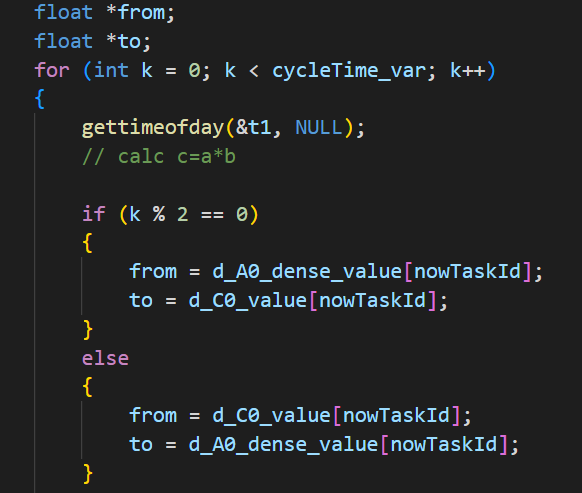
\includegraphics[width=0.5\textwidth]{cyc.png}
\end{figure}
Thus,we killed the memcpy function call inside the cycle,which really made a lot contribution on performance.

\subsection{Parallelize reLU}
At first,reLU function was called single-threaded.However,reLU depends on nothing rather than the matrix to be reLUed.So just define the grid and block and parallelize it.
\begin{figure}[H]
    \centering
    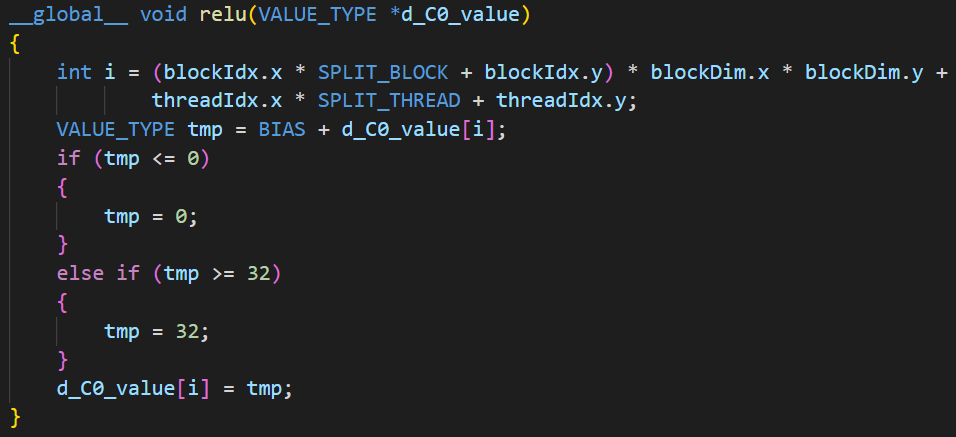
\includegraphics[width=0.6\textwidth]{rrr.png}
    \caption{reLU function implement}
\end{figure}
\begin{figure}[H]
    \centering
    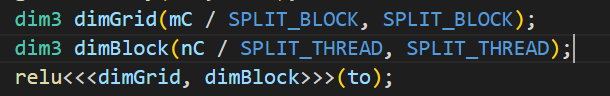
\includegraphics[width=0.5\textwidth]{re.png}
    \caption{reLU function call}
\end{figure}
\subsection{Hoisting}
When batch size set small,about 2000,a problem will occur that time consumption each layer cost will increase to another const.Conjecture is that too much temp variables are put into the for loop,and I never free them until error occur.So hoist them out of for loop solved the problem.
\subsection{Warm up}
Sometimes,the running time doesn't performs very stable.The first calculation will cost much more time than others.So,a warm up maybe needed.

Just call the calc function and limit the cycle time,that's ok.Also,the matrix A will be set to initial for the correct answer.
\begin{figure}[H]
    \centering
    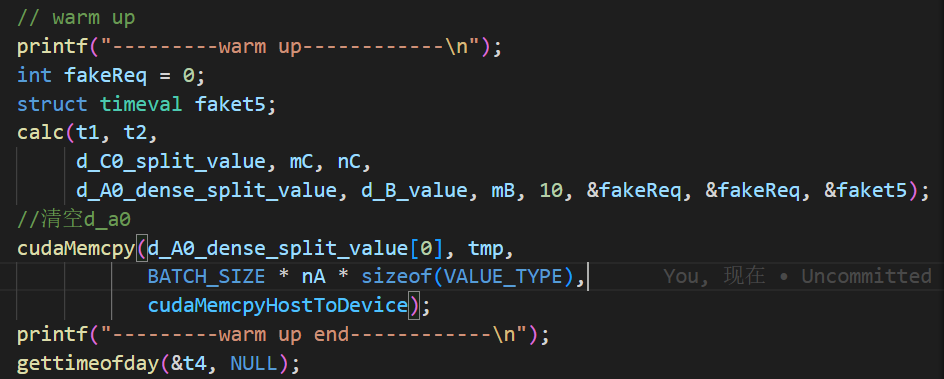
\includegraphics[width=0.8\textwidth]{dasf.png}
    \caption{warm up}
\end{figure}
\section{Final Result}
Actually I tried some cases like set the batch size to a very small size and treat CPU and GPU two device to make full use of them,or generate several processes in one node to exploit full performance of the machine.However,no one was better than just one process and no CPU exploitation.So here I will only give you two version of result,one is one node,and another is two nodes.

However,this project actually can be run in any number of nodes and register new device in any time,just like bitcoin mining.

The time consumption actually is the greatest one shown in each process.Since the master process,or the dealer will end count at the end of 115th calculation cycle rather the actual end of calculation,since the dealer will end count when every slaver request a END\_CALC single.

So,the actual performance of one node is 5809ms,and the performance of two nodes is 2996ms.
\begin{figure}[H]
    \centering
    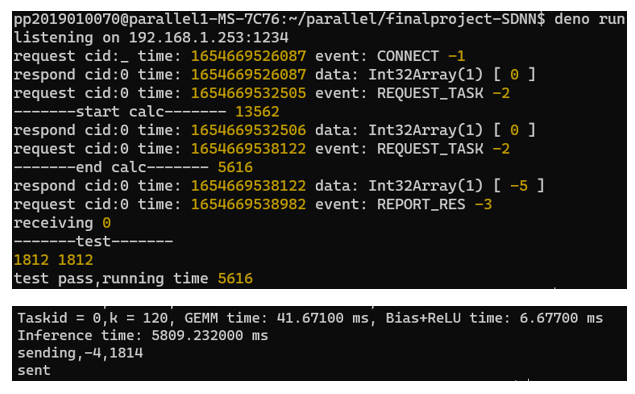
\includegraphics[width=0.8\textwidth]{one.png}
    \caption{one node}
    \label{}
\end{figure}
\begin{figure}[H]
    \centering
    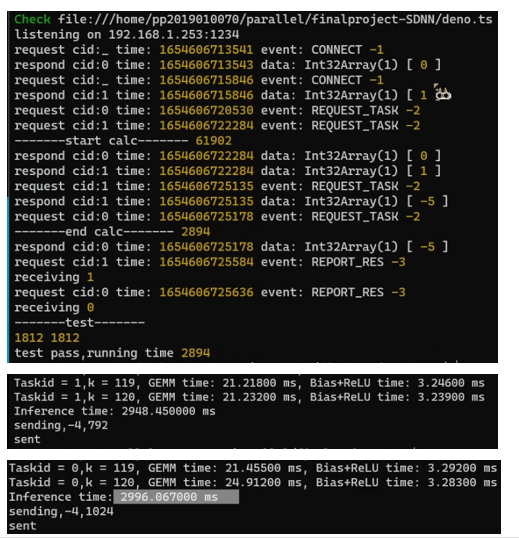
\includegraphics[width=0.8\textwidth]{two.png}
    \caption{two nodes}
    \label{}
\end{figure}
\section{Appendix}
All source codes are stored in the GitHub repository:


\url{https://github.com/BI1LQV/parallel/tree/master/finalproject-SDNN/}
\end{document}